\section{The CnC Programming Model}

Concurrent Collections (CnC) is one such data-centric programming
model, the deterministic semantics of which allow a task-based runtime
to programmatically exploit parallelism. In this model, algorithms are
designed based on their data and control dependencies
~\cite{budimlicconcurrent}. The specifics regarding the execution of
the algorithm is then abstracted out of the implementation. This
allows the runtime to optimally decide when and where to schedule
computation. Hints can also be provided to the runtime through a
separate file called a ``tuning specification''.

The CnC model is built on three key constructs: step collections, data collections, and control collections ~\cite{budimlicconcurrent}.  A step collection defines computation, an instance of which consumes and produces data.  The consumed and produced data, or data items, belong to data collections.  Data items within a data collection are indexed using item tags.
%% RRL: We need to say more about tags.
Finally the control collection describes the prescription, or creation, of step instances.  The relationship between these three collections is defined statically in an input file called a ``CnC graph''.

Developing a CnC application begins with designing the CnC graph file.  An algorithm is broken down into computation steps, instances of which correspond to different input arguments.  These steps along with the data collections become nodes in a graph.  Each step can optionally consume data, produce data, and prescribe additional computation.  These relationships, producer, consumer, and control, define the edges in the graph and will dynamically be satisfied as the program executes.

\begin{figure*}[!htb]
  \centering
  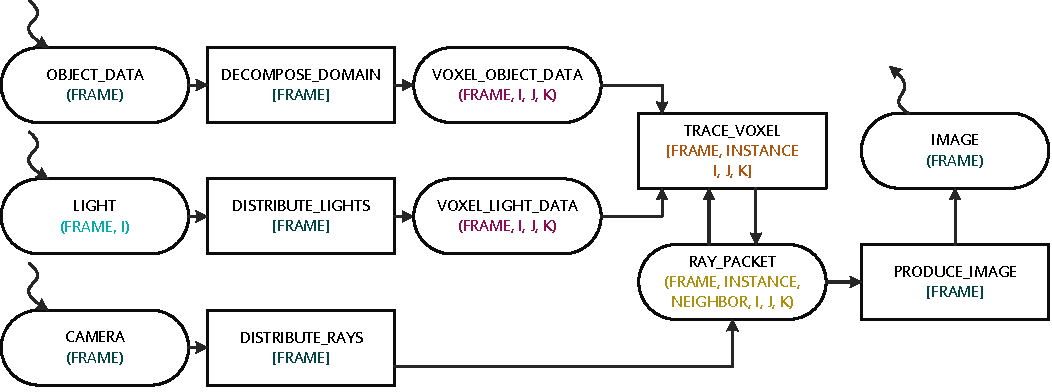
\includegraphics[width=\textwidth]{drawings/CnC.pdf}
  \caption{CnC Graph.}
  \label{fig:cnc}
\end{figure*}
%% RRL: We need to say more about this diagram.

The next and final required step in producing a CnC application is to implement the step logic.  The flow within a single CnC step is as follows: consume, compute, and produce.  This ordering is required as there is no guarantee the data a step needs will be ready when the step beings executing.  Internally, CnC will attempt to retrieve the data, if it is not ready, the step will halt execution and try again later.  To improve performance, hints can be provided through the tuning specification to ensure steps are only prescribed and scheduled for execution when their required input data is ready.
%% RRL: It seems odd that so necessary a consideration that a step
%% needs to have its data ready before it starts running is considered
%% ``tuning''.

%%% Local Variables: 
%%% mode: latex
%%% TeX-master: "main"
%%% End: 
